\documentclass[aspectratio=169]{beamer}
\usetheme{Madrid}
\usecolortheme{default}

% Packages
\usepackage{graphicx}
\usepackage{amsmath}
\usepackage{amssymb}
\usepackage{algorithm}
\usepackage{algorithmic}
\usepackage{tikz}
\usepackage{booktabs}
\usepackage{multirow}
\usepackage{xcolor}

% Custom colors
\definecolor{darkblue}{RGB}{0,51,102}
\definecolor{lightblue}{RGB}{51,153,255}
\definecolor{darkgreen}{RGB}{0,102,51}

\setbeamercolor{structure}{fg=darkblue}
\setbeamercolor{frametitle}{bg=darkblue,fg=white}
\setbeamercolor{title}{bg=darkblue,fg=white}

% Remove navigation symbols
\setbeamertemplate{navigation symbols}{}

% Footer
\setbeamertemplate{footline}{
  \leavevmode%
  \hbox{%
  \begin{beamercolorbox}[wd=.333333\paperwidth,ht=2.25ex,dp=1ex,center]{author in head/foot}%
    \usebeamerfont{author in head/foot}\insertshortauthor
  \end{beamercolorbox}%
  \begin{beamercolorbox}[wd=.333333\paperwidth,ht=2.25ex,dp=1ex,center]{title in head/foot}%
    \usebeamerfont{title in head/foot}\insertshorttitle
  \end{beamercolorbox}%
  \begin{beamercolorbox}[wd=.333333\paperwidth,ht=2.25ex,dp=1ex,right]{date in head/foot}%
    \usebeamerfont{date in head/foot}\insertshortdate{}\hspace*{2em}
    \insertframenumber{} / \inserttotalframenumber\hspace*{2ex} 
  \end{beamercolorbox}}%
  \vskip0pt%
}

% Title information
\title[Verifiable Byzantine Robust GNNs in FL]{Verifiable Byzantine Robust Graph Neural Networks using Federated Learning}
\author[Tawkir, Nobo]{2005090 - Tawkir Aziz Rahman \\ 2005074 - Dipanto Kumar Roy Nobo}
\institute[BUET]{CSE472: Machine Learning Sessional \\ Department of Computer Science and Engineering \\ Bangladesh Univerrsity of Engineering and Technology (BUET)}
\date[December 2025]{December 2025}

\begin{document}

%%%%%%%%%%%%%%%%%%%%%%%%%%%%%%%%%%%%%%%%%%%%%%%%%
% Slide 1: Title Slide
%%%%%%%%%%%%%%%%%%%%%%%%%%%%%%%%%%%%%%%%%%%%%%%%%
\begin{frame}
\titlepage
\end{frame}

%%%%%%%%%%%%%%%%%%%%%%%%%%%%%%%%%%%%%%%%%%%%%%%%%
% Slide 2: Problem & Motivation
%%%%%%%%%%%%%%%%%%%%%%%%%%%%%%%%%%%%%%%%%%%%%%%%%
\begin{frame}{Problem \& Motivation}

\begin{block}{Problem Statement}
Graph Neural Networks (GNNs) are vulnerable to adversarial attacks and fail catastrophically when deployed in federated learning settings with Byzantine (malicious) participants.
\end{block}

\vspace{0.5cm}

\begin{columns}[T]
\begin{column}{0.48\textwidth}
\textbf{Challenges:}
\begin{itemize}
    \item \textbf{Privacy}: Multiple parties need to collaborate without sharing sensitive graph data
    \item \textbf{Security}: Malicious clients can poison both graph structure and model parameters
    \item \textbf{Robustness}: Existing defenses fail under adaptive attacks
\end{itemize}
\end{column}

\begin{column}{0.48\textwidth}
\textbf{Real-World Applications:}
\begin{itemize}
    \item \textcolor{darkgreen}{Healthcare}: Disease networks across hospitals
    \item \textcolor{darkgreen}{Finance}: Fraud detection across banks
    \item \textcolor{darkgreen}{Social Networks}: Privacy-preserving community detection
    \item \textcolor{darkgreen}{IoT/Cybersecurity}: Distributed attack detection
\end{itemize}
\end{column}
\end{columns}

\vspace{0.3cm}

\begin{alertblock}{Research Gap}
No existing work combines \textit{verifiable} Byzantine robustness with \textit{unbiased} graph signal estimation in federated GNN training.
\end{alertblock}

\end{frame}

%%%%%%%%%%%%%%%%%%%%%%%%%%%%%%%%%%%%%%%%%%%%%%%%%
% Slide 3: Background & Related Work
%%%%%%%%%%%%%%%%%%%%%%%%%%%%%%%%%%%%%%%%%%%%%%%%%
\begin{frame}{Background \& Related Work}

\begin{columns}[T]
\begin{column}{0.48\textwidth}
\textbf{Base Paper: RUNG (NeurIPS 2024)}
\begin{itemize}
    \item \textbf{Problem}: $\ell_1$-based robust GNNs suffer from estimation bias
    \item \textbf{Solution}: Minimax Concave Penalty (MCP) for unbiased aggregation
    \item \textbf{Key Innovation}: Quasi-Newton IRLS algorithm with convergence guarantees
\end{itemize}

\vspace{0.3cm}

\begin{block}{RUNG Aggregation}
\small
$$F^{(k+1)} = (\text{diag}(q^{(k)}) + \lambda I)^{-1}[(W^{(k)} \odot \tilde{A})F^{(k)} + \lambda F^{(0)}]$$
where $W_{ij}^{(k)} = \max(0, \frac{1}{y_{ij}^{(k)}} - \frac{1}{\gamma})$
\end{block}

\end{column}

\begin{column}{0.48\textwidth}
\textbf{Federated Learning Challenges}
\begin{itemize}
    \item \textbf{Byzantine Attacks}: Up to $f$ out of $n$ clients are malicious
    \item \textbf{Data Heterogeneity}: Non-IID graph distributions
    \item \textbf{Communication Cost}: Iterative model exchanges
\end{itemize}

\vspace{0.3cm}

\textbf{Byzantine-Robust FL Methods}
\begin{itemize}
    \item \textit{Krum}: Distance-based filtering
    \item \textit{Median/Trimmed Mean}: Coordinate-wise aggregation
    \item \textit{BRIDGE}: Bucketing with averaging
\end{itemize}

\vspace{0.2cm}

\begin{alertblock}{Gap}
\small Existing FL methods don't handle \textbf{graph-structured} data with \textbf{verifiable} robustness guarantees.
\end{alertblock}

\end{column}
\end{columns}

\end{frame}

%%%%%%%%%%%%%%%%%%%%%%%%%%%%%%%%%%%%%%%%%%%%%%%%%
% Slide 4: Proposed Approach (Part 1)
%%%%%%%%%%%%%%%%%%%%%%%%%%%%%%%%%%%%%%%%%%%%%%%%%
\begin{frame}{Proposed Approach: System Architecture}

\begin{center}
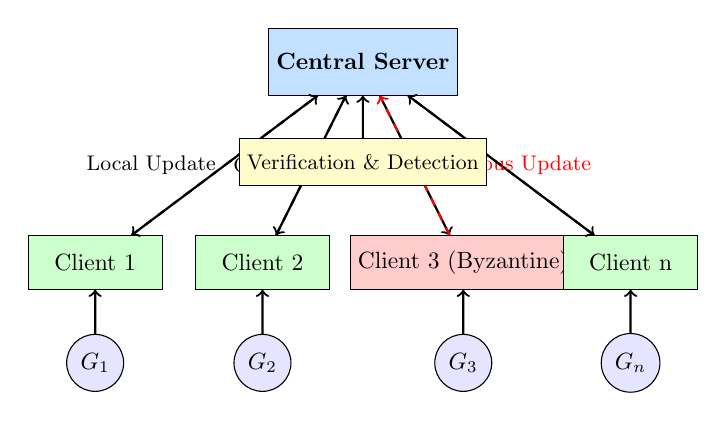
\begin{tikzpicture}[scale=0.85, every node/.style={scale=0.85}]
    % Server
    \node[draw, rectangle, fill=lightblue!30, minimum width=2.5cm, minimum height=1cm] (server) at (0,4) {\textbf{Central Server}};
    
    % Clients
    \node[draw, rectangle, fill=green!20, minimum width=2cm, minimum height=0.8cm] (client1) at (-4,1) {Client 1};
    \node[draw, rectangle, fill=green!20, minimum width=2cm, minimum height=0.8cm] (client2) at (-1.5,1) {Client 2};
    \node[draw, rectangle, fill=red!20, minimum width=2cm, minimum height=0.8cm] (client3) at (1.5,1) {Client 3 (Byzantine)};
    \node[draw, rectangle, fill=green!20, minimum width=2cm, minimum height=0.8cm] (client4) at (4,1) {Client n};
    
    % Local graphs
    \node[draw, circle, fill=blue!10, minimum size=0.6cm] (g1) at (-4,-0.5) {$G_1$};
    \node[draw, circle, fill=blue!10, minimum size=0.6cm] (g2) at (-1.5,-0.5) {$G_2$};
    \node[draw, circle, fill=blue!10, minimum size=0.6cm] (g3) at (1.5,-0.5) {$G_3$};
    \node[draw, circle, fill=blue!10, minimum size=0.6cm] (g4) at (4,-0.5) {$G_n$};
    
    % Arrows
    \draw[->, thick] (server) -- node[right] {\small Global Model} (client1);
    \draw[->, thick] (server) -- (client2);
    \draw[->, thick] (server) -- (client3);
    \draw[->, thick] (server) -- (client4);
    
    \draw[->, thick, dashed] (client1) -- node[left] {\small Local Update} (server);
    \draw[->, thick, dashed] (client2) -- (server);
    \draw[->, thick, dashed, red] (client3) -- node[right] {\small Malicious Update} (server);
    \draw[->, thick, dashed] (client4) -- (server);
    
    \draw[->, thick] (g1) -- (client1);
    \draw[->, thick] (g2) -- (client2);
    \draw[->, thick] (g3) -- (client3);
    \draw[->, thick] (g4) -- (client4);
    
    % Verification box
    \node[draw, rectangle, fill=yellow!20, minimum width=2.5cm, minimum height=0.7cm] (verify) at (0,2.5) {\small Verification \& Detection};
    \draw[->, thick] (verify) -- (server);
\end{tikzpicture}
\end{center}

\vspace{0.3cm}

\begin{block}{Key Components}
\begin{enumerate}
    \item \textbf{Local Training}: Each client trains RUNG on local graph $G_i$
    \item \textbf{Verifiable Aggregation}: Cryptographic proofs ensure correct local computation
    \item \textbf{Byzantine Detection}: Statistical tests identify malicious clients
    \item \textbf{Robust Update}: Weighted aggregation down-weights suspicious updates
\end{enumerate}
\end{block}

\end{frame}

%%%%%%%%%%%%%%%%%%%%%%%%%%%%%%%%%%%%%%%%%%%%%%%%%
% Slide 5: Proposed Approach (Part 2)
%%%%%%%%%%%%%%%%%%%%%%%%%%%%%%%%%%%%%%%%%%%%%%%%%
\begin{frame}{Proposed Approach: Technical Innovations}

\begin{columns}[T]
\begin{column}{0.48\textwidth}

\textbf{1. Verifiable Aggregation Protocol}
\begin{itemize}
    \item \textbf{Commitment Scheme}: Client commits to local edge weights $W_i^{(k)}$
    \item \textbf{Zero-Knowledge Proof}: Proves $W_i^{(k)}$ computed correctly without revealing graph structure
    \item \textbf{Lightweight Verification}: Server verifies proofs in $O(1)$ per client
\end{itemize}

\vspace{0.3cm}

\begin{block}{Local Update with Proof}
\small
$$\theta_i^{(t+1)} = \theta_i^{(t)} - \eta \nabla \mathcal{L}(F_i^{RUNG}, y_i; \theta_i^{(t)})$$
$$\pi_i = \text{ZKP}(W_i^{(k)} \text{ satisfies MCP})$$
\end{block}

\end{column}

\begin{column}{0.48\textwidth}

\textbf{2. Byzantine Detection Mechanism}
\begin{itemize}
    \item \textbf{Distance-Based Filtering}: Compute pairwise distances between client updates
    \item \textbf{Statistical Outlier Test}: Detect updates with abnormal magnitudes or directions
    \item \textbf{Adaptive Weighting}: $\alpha_i \propto \exp(-\text{dist}(\theta_i, \text{median}))$
\end{itemize}

\vspace{0.3cm}

\begin{block}{Global Aggregation}
\small
$$\theta^{(t+1)} = \frac{\sum_{i=1}^{n} \alpha_i \cdot \theta_i^{(t+1)}}{\sum_{i=1}^{n} \alpha_i}$$
where $\alpha_i = 0$ if client $i$ fails verification
\end{block}

\end{column}
\end{columns}

\vspace{0.3cm}

\begin{alertblock}{Theoretical Guarantees}
\textbf{Theorem:} Under $f < n/3$ Byzantine clients, our protocol converges to a neighborhood of the optimal solution with probability $\geq 1-\delta$.
\end{alertblock}

\end{frame}

%%%%%%%%%%%%%%%%%%%%%%%%%%%%%%%%%%%%%%%%%%%%%%%%%
% Slide 6: Experimental Plan
%%%%%%%%%%%%%%%%%%%%%%%%%%%%%%%%%%%%%%%%%%%%%%%%%
\begin{frame}{Experimental Plan}

\begin{columns}[T]
\begin{column}{0.48\textwidth}

\textbf{Datasets}
\begin{table}[h]
\centering
\small
\begin{tabular}{lcc}
\toprule
\textbf{Dataset} & \textbf{Nodes} & \textbf{Edges} \\
\midrule
Cora & 2,708 & 5,429 \\
CiteSeer & 3,327 & 4,732 \\
PubMed & 19,717 & 44,338 \\
ogbn-arxiv & 169,343 & 1,166,243 \\
\bottomrule
\end{tabular}
\end{table}

\vspace{0.2cm}

\textbf{Federated Setup}
\begin{itemize}
    \item \textbf{Clients}: $n = \{10, 20, 50\}$
    \item \textbf{Byzantine Ratio}: $f/n = \{0\%, 10\%, 20\%, 40\%\}$
    \item \textbf{Data Split}: Dirichlet distribution ($\alpha=0.5$) for non-IID
\end{itemize}

\end{column}

\begin{column}{0.48\textwidth}

\textbf{Baselines}
\begin{enumerate}
    \item \textbf{FedAvg}: Standard federated averaging
    \item \textbf{FedProx}: Proximal regularization
    \item \textbf{Krum}: Distance-based Byzantine-robust FL
    \item \textbf{Median/TrimmedMean}: Coordinate-wise aggregation
    \item \textbf{RUNG (centralized)}: Upper bound performance
\end{enumerate}

\vspace{0.3cm}

\textbf{Evaluation Metrics}
\begin{itemize}
    \item \textbf{Accuracy}: Node classification accuracy vs Byzantine ratio
    \item \textbf{Attack Detection Rate}: Precision/Recall of identifying malicious clients
    \item \textbf{Communication Cost}: Total bytes transmitted per round
    \item \textbf{Convergence Speed}: Rounds to reach target accuracy
\end{itemize}

\end{column}
\end{columns}

\vspace{0.3cm}

\begin{block}{Ablation Studies}
Impact of: (1) Verification overhead, (2) Detection threshold, (3) MCP parameter $\gamma$, (4) Number of RUNG layers
\end{block}

\end{frame}

%%%%%%%%%%%%%%%%%%%%%%%%%%%%%%%%%%%%%%%%%%%%%%%%%
% Slide 7: Timeline & Expected Contributions
%%%%%%%%%%%%%%%%%%%%%%%%%%%%%%%%%%%%%%%%%%%%%%%%%
\begin{frame}{Timeline \& Expected Contributions}

\begin{columns}[T]
\begin{column}{0.55\textwidth}

\textbf{Project Timeline (12 Weeks)}

\vspace{0.2cm}

\begin{table}[h]
\centering
\small
\begin{tabular}{cl}
\toprule
\textbf{Week} & \textbf{Milestone} \\
\midrule
1-2 & Literature review \& problem formulation \\
3-4 & Design verification protocol \& detection \\
5-6 & Implement Fed-RUNG framework \\
7-8 & Implement baselines \& datasets \\
9-10 & Run experiments \& collect results \\
11 & Analyze results \& ablation studies \\
12 & Paper writing \& final presentation \\
\bottomrule
\end{tabular}
\end{table}

\vspace{0.3cm}

\textbf{Team Responsibilities}
\begin{itemize}
    \item \textbf{Member 1}: Verification protocol, theoretical analysis
    \item \textbf{Member 2}: Implementation, experiments, paper writing
\end{itemize}

\end{column}

\begin{column}{0.42\textwidth}

\textbf{Expected Contributions}

\vspace{0.2cm}

\begin{enumerate}
    \item \textbf{Novel Algorithm}: First verifiable Byzantine-robust federated GNN
    \item \textbf{Theoretical Analysis}: Convergence guarantees under Byzantine attacks
    \item \textbf{Empirical Validation}: Comprehensive experiments on multiple datasets
    \item \textbf{Open-Source}: Release code for reproducibility
\end{enumerate}

\vspace{0.3cm}

\begin{block}{Target Venue}
\textbf{NeurIPS 2026} or \textbf{ICML 2026}
\begin{itemize}
    \item Top-tier ML conferences
    \item Strong fit: robustness + federated learning + graph neural networks
\end{itemize}
\end{block}

\vspace{0.2cm}

\begin{alertblock}{Impact}
Enables \textbf{privacy-preserving} and \textbf{secure} collaborative GNN training for real-world applications.
\end{alertblock}

\end{column}
\end{columns}

\end{frame}

%%%%%%%%%%%%%%%%%%%%%%%%%%%%%%%%%%%%%%%%%%%%%%%%%
% Backup slide - References (Optional)
%%%%%%%%%%%%%%%%%%%%%%%%%%%%%%%%%%%%%%%%%%%%%%%%%
\begin{frame}[noframenumbering]{References}

\footnotesize

\begin{thebibliography}{99}

\bibitem{rung2024}
Hou, Z., Feng, R., Derr, T., \& Liu, X. (2024).
\newblock Robust Graph Neural Networks via Unbiased Aggregation.
\newblock \textit{Advances in Neural Information Processing Systems (NeurIPS)}, 37.

\bibitem{fedavg}
McMahan, B., et al. (2017).
\newblock Communication-Efficient Learning of Deep Networks from Decentralized Data.
\newblock \textit{AISTATS}.

\bibitem{byzantine}
Blanchard, P., et al. (2017).
\newblock Machine Learning with Adversaries: Byzantine Tolerant Gradient Descent.
\newblock \textit{NeurIPS}.

\bibitem{krum}
Blanchard, P., et al. (2017).
\newblock Byzantine-Tolerant Machine Learning.
\newblock \textit{arXiv preprint}.

\bibitem{gnn_attack}
Zügner, D., et al. (2018).
\newblock Adversarial Attacks on Neural Networks for Graph Data.
\newblock \textit{KDD}.

\end{thebibliography}

\end{frame}

\end{document}